\chapter{実現方法}\label{chap:method}

ARマーカーを用いずに原点を調整する手法として、マップ画像を用いて手動で調整する手法を提案する。


\section{内部情報の取得}

ロボットの内部情報の取得には、ROS#を用いた。
ROS#とは、Unity上でROSを利用できるようにするパケージで、UnityとROSでデータの通信が可能になる。
また、取得したデータは数値データであるため、可視化の作業もROS#を用いて行っている。
図\ref{VisRosUni}は、RvizとUnityでセンサーの可視化を行った様子である。
図\ref{VisRosUni}から、UnityでもRvizと同じような可視化結果が出力できていることが確認できる。


\begin{figure}[H]
  \begin{minipage}[b]{0.45\linewidth}
    \centering
    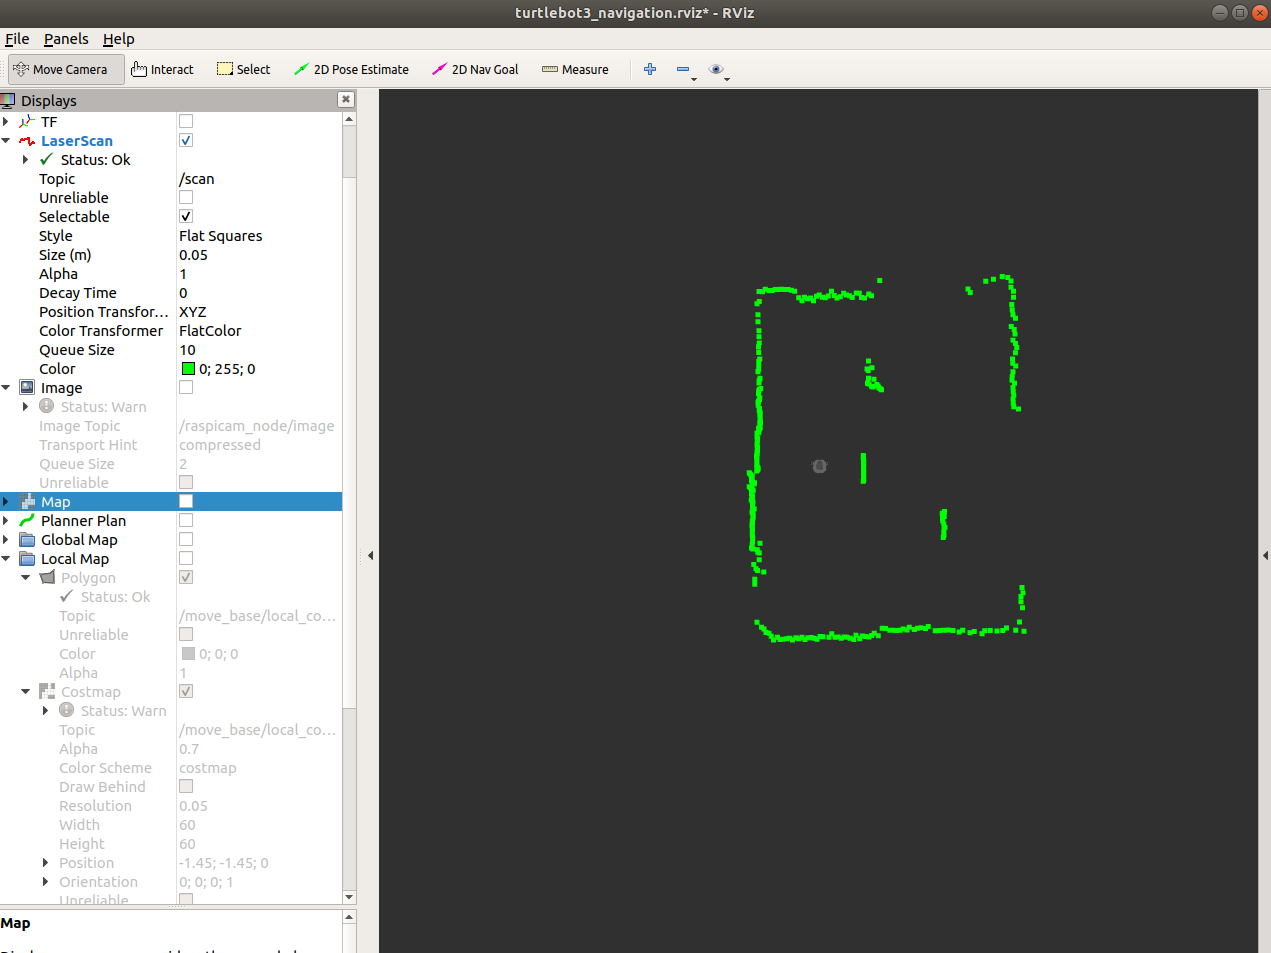
\includegraphics[keepaspectratio, width=.9\hsize]{figs/Rviz_Lidar.png}
    \subcaption{Rviz上での可視化}
  \end{minipage}
  \begin{minipage}[b]{0.45\linewidth}
    \centering
    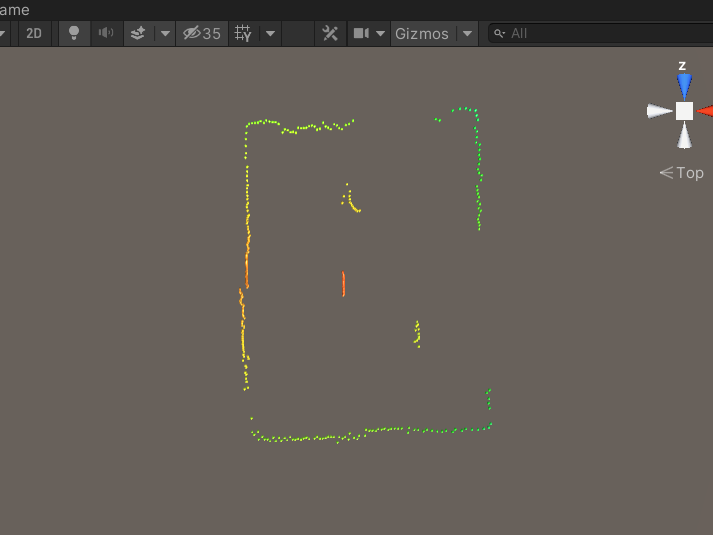
\includegraphics[keepaspectratio, width=.9\hsize]{figs/Unity_Lidar.png}
    \subcaption{Unity上での可視化}
  \end{minipage}
  \caption{データの可視化}\label{VisRosUni}
\end{figure}


\section{ARでの可視化}

Unity上で可視化したデータをARで表示するために、ARcoreを利用した。
ARcoreとは、Googleが提供するARプラットフォームであり、端末のトラッキングやオブジェクトの配置ができる。
トラッキングには、Visual Odometryという画像の特徴点から端末の移動量を推定する技術が利用されている。


\section{原点の調整}

マーカレスで原点の調整を行う手法は、自己位置推定に用いるマップを利用した手法を提案する。
AR上にマップを表示し、マップと現実空間を合わせることで原点の調整を行う。
図\ref{ARpoint}は、原点の調整の様子である。
図\ref{ARpointmiss}では、地図上の障害物、現実空間の障害物がずれていることがわかる。
このずれを、図\ref{ARpointtrue}のように合わせることで原点の調整を行う。


\begin{figure}[H]
  \begin{minipage}[b]{0.45\linewidth}
    \centering
    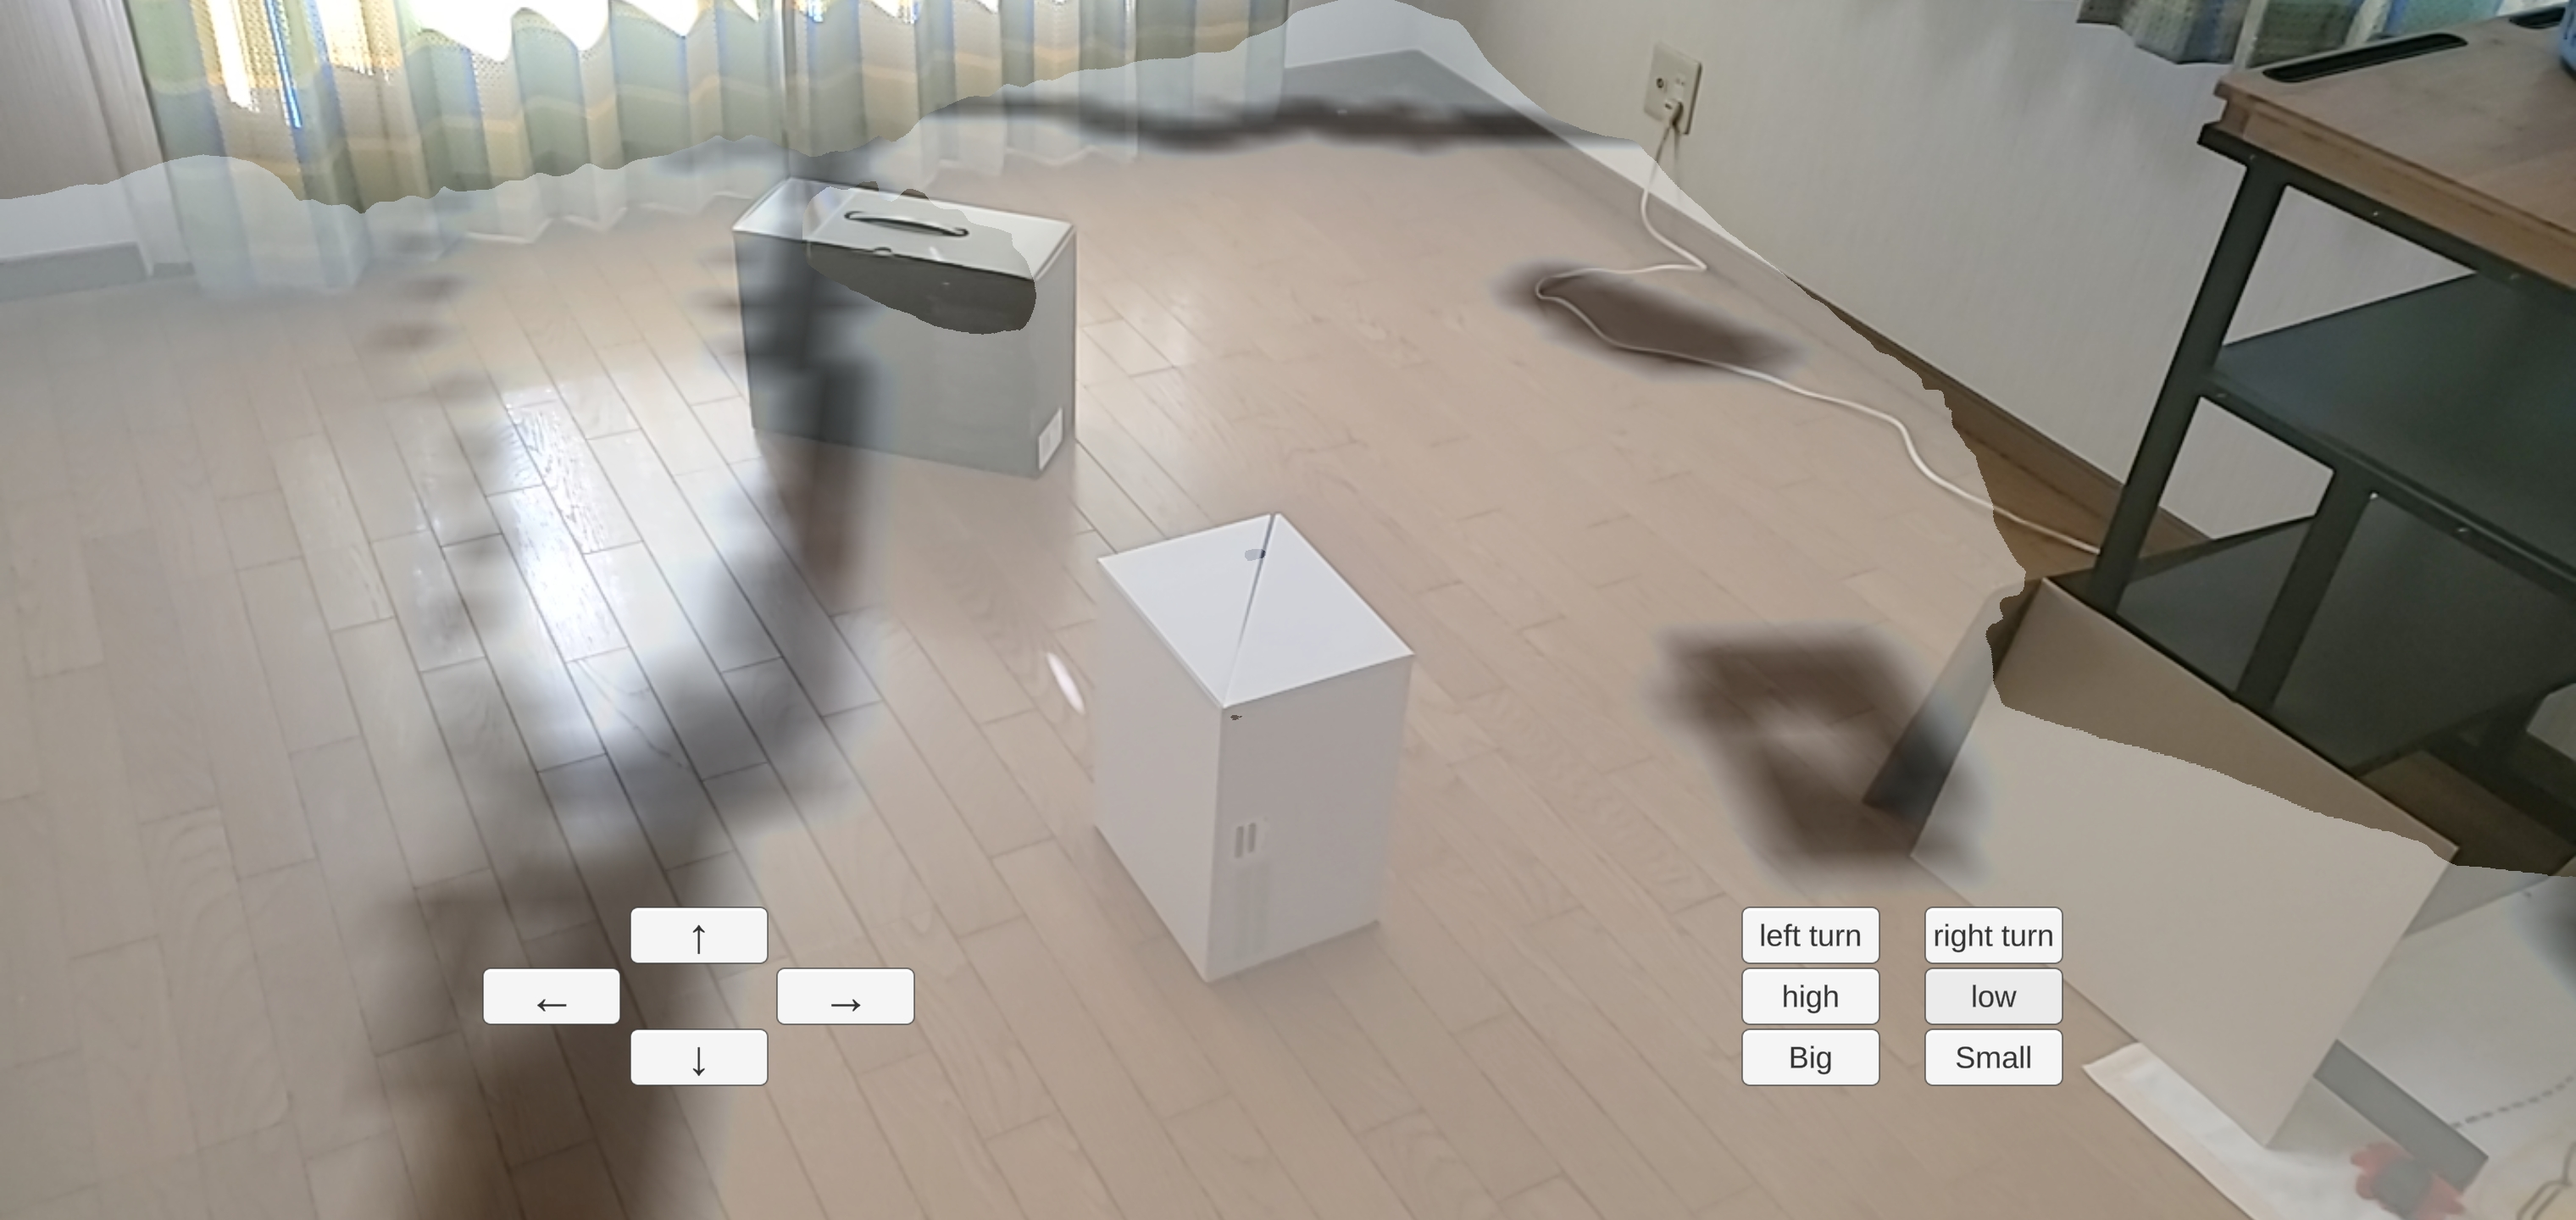
\includegraphics[keepaspectratio, width=.9\hsize]{figs/ARmiss.jpg}
    \subcaption{原点がずれた状態}\label{ARpointmiss}
  \end{minipage}
  \begin{minipage}[b]{0.45\linewidth}
    \centering
    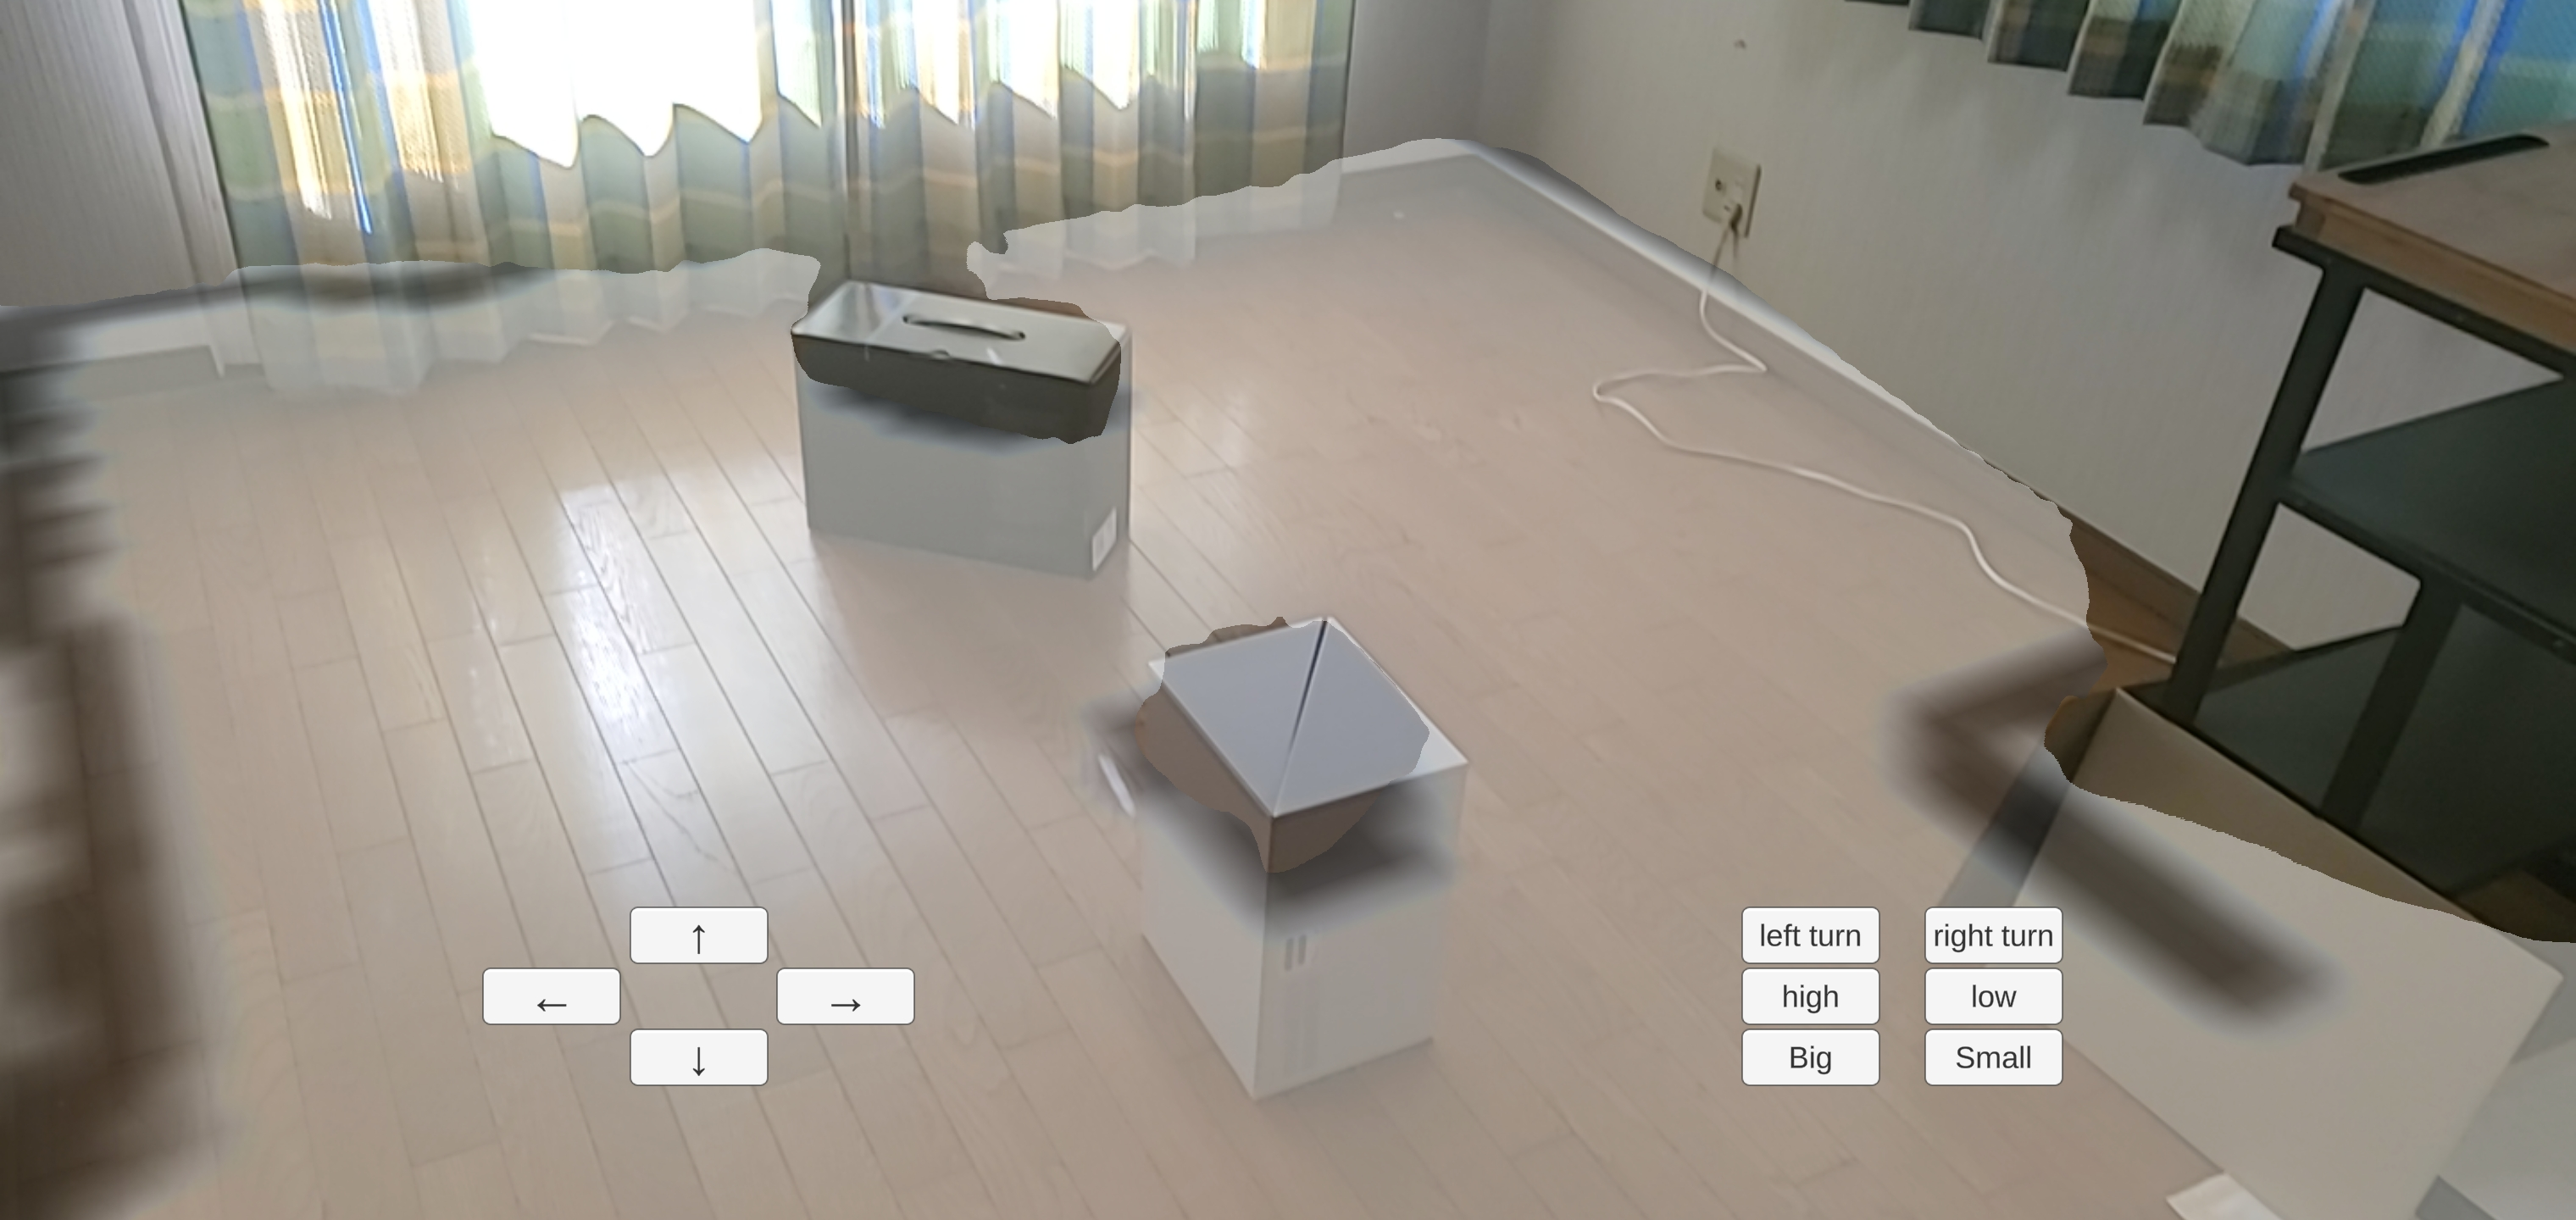
\includegraphics[keepaspectratio, width=.9\hsize]{figs/ARtrue.jpg}
    \subcaption{原点を合わせた状態}\label{ARpointtrue}
  \end{minipage}
  \caption{原点の調整}\label{ARpoint}
\end{figure}